Let
\[
\Omega=\left\{(x,y):\,0\le x\le 1,\,0\le y\le 1\right\}
\]
and let $f(x,y,t) = (x-{1 \over 2})^3 (y-{1 \over 2}) e^{-t}$. Note that, for $m,n=1,2,\ldots$,
\[
\int_0^1 \int_0^1 2 f(x,y,t) \sin(m \pi x) \sin(n \pi y)\,dx\,dy= {(1+(-1)^m)(1+(-1)^n) (m^2\pi^2-24)\over 8 m^3 n \pi^4} e^{-t}.
\]
In this question we will consider the problem of finding the solution $u(x,y,t)$ to the heat equation
\[ 
u_t(x,y,t)-(u_{xx}(x,y,t) +u_{yy}(x,y,t)) = f(x,y,t), \qquad 0\le x \le 1, \quad 0\le y\le 1, \quad t\ge 0,
\]
with homogeneous Dirichlet boundary conditions
\[
u(x,0,t)=u(x,1,t)=u(0,y,t)=u(1,y,t)=0, \qquad 0\le x \le 1, \quad 0\le y\le 1, \quad t\ge 0,
\]
and initial condition
\[
u(x,y,0) = 0, \qquad 0\le x\le 1, \quad 0\le y\le 1.
\]
Let
\[
C^2_D(\Omega)=\left\{v\in C^2(\Omega):\,v(x,0)=v(x,1)=v(0,y)=v(1,y)=0,\,0\le x\le 1,\,0\le y\le 1\right\}.
\]
Let the linear operator $L:\,C^2_D(\Omega)\rightarrow C(\Omega)$ be defined by
\[
\left(L v\right)(x,y) = -\left(v_{xx}(x,y) + v_{yy}(x,y)\right).
\]
The operator $L$ has eigenvalues $\lambda_{j,k}\in\R$ and eigenfunctions
\[
\psi_{j,k}(x,y) = 2 \sin(j \pi x) \sin(k \pi y)
\]
for $j,k = 1,2,\ldots$, which are such that
\[
L\psi_{j,k}=\lambda_{j,k}\psi_{j,k}
\]
for $j,k = 1,2,\ldots$. Recall that in Homework 40 you obtained a formula for $\lambda_{j,k}$ for $j,k = 1,2,\ldots$.

\begin{enumerate}
\item We can write
\[
u(x,y,t) = \sum_{j=1}^\infty \sum_{k=1}^\infty a_{j,k}(t) \psi_{j,k} (x,y)
\]
and
\[
f(x,y,t) = \sum_{j=1}^\infty \sum_{k=1}^\infty c_{j,k}(t) \psi_{j,k} (x,y)
\]
where
\[
c_{j,k}(t) = \int_0^1 \int_0^1 f(x,y,t) \psi_{j,k} (x,y)\,dx\,dy.
\]
What ordinary differential equation and initial condition does $a_{j,k}(t)$ satisfy for $j,k = 1,2,\ldots$?
\\
\item Obtain an expression for $a_{j,k}(t)$ for $j,k=1,2,\ldots$.
\\
\item Use you answer to part~(b) to write out a formula for $u(x,y,t)$.
\\
\item Plot
\[
u_{15}(x,y,t) = \sum_{j=1}^{15} \sum_{k=1}^{15}a_{j.k}(t)\psi_{j,k}(x,y)
\]
at the four times $t=0, 0.005, 0.1, 2$. Use the command \verb|zlim([-.00016 .00016])| so that the axes on all of your plots are the same. Your plot for $t=0.1$ should resemble the plot below.

\begin{center}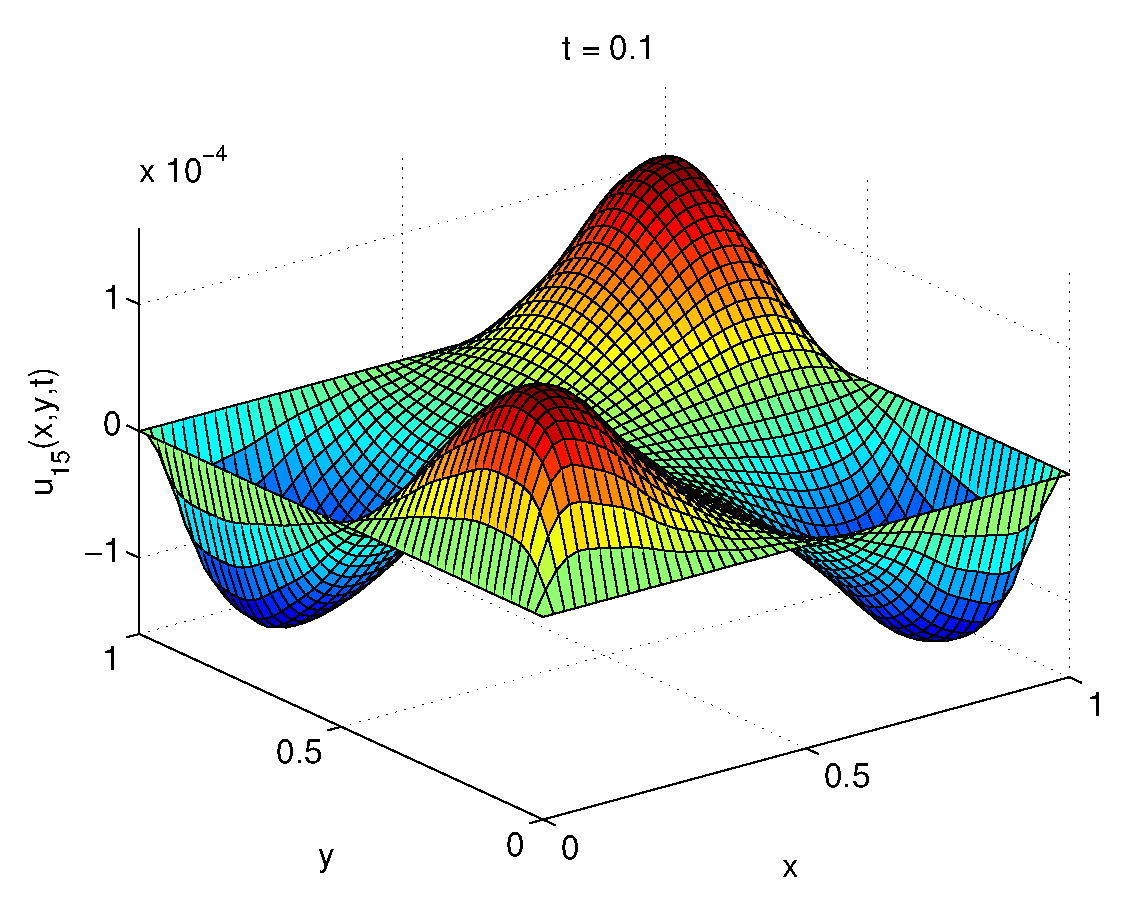
\includegraphics[scale=0.6]{heat2d3} \end{center}
\end{enumerate}


%%%%%%%%%%%%%%%%%%%%%%%%%%%%%%%%%%%%%%%%%%%%%%%%%%%%%%%%%%%%%%%%%%%%%%%%%%%%%%%%

\ifthenelse{\boolean{showsols}}{\input heat2d_sol}{}

